\documentclass[]{article}
    \usepackage{lmodern}
    \usepackage{amssymb,amsmath}
\usepackage{ifxetex,ifluatex}
\usepackage{fixltx2e} % provides \textsubscript
\ifnum 0\ifxetex 1\fi\ifluatex 1\fi=0 % if pdftex
\usepackage[T1]{fontenc}
\usepackage[utf8]{inputenc}
  \else % if luatex or xelatex
\ifxetex
\usepackage{mathspec}
\usepackage{xltxtra,xunicode}
\else
  \usepackage{fontspec}
\fi
\defaultfontfeatures{Mapping=tex-text,Scale=MatchLowercase}
\newcommand{\euro}{€}
        \fi
% use upquote if available, for straight quotes in verbatim environments
\IfFileExists{upquote.sty}{\usepackage{upquote}}{}
% use microtype if available
\IfFileExists{microtype.sty}{%
  \usepackage{microtype}
  \UseMicrotypeSet[protrusion]{basicmath} % disable protrusion for tt fonts
}{}
  \usepackage[right=1in,top=1.25in,bottom=1.25in,left=2.5in]{geometry}
  \ifxetex
\usepackage[setpagesize=false, % page size defined by xetex
            unicode=false, % unicode breaks when used with xetex
            xetex]{hyperref}
\else
  \usepackage[unicode=true]{hyperref}
\fi
\hypersetup{breaklinks=true,
bookmarks=true,
pdfauthor={},
pdftitle={Preregistration for reproducing Gooding et al.~2009},
colorlinks=true,
citecolor=blue,
urlcolor=blue,
linkcolor=magenta,
pdfborder={0 0 0}}
\urlstyle{same}  % don't use monospace font for urls
\setlength{\parindent}{0pt}
\setlength{\parskip}{6pt plus 2pt minus 1pt}
\setlength{\emergencystretch}{3em}  % prevent overfull lines
\providecommand{\tightlist}{%
\setlength{\itemsep}{0pt}\setlength{\parskip}{0pt}}
\setcounter{secnumdepth}{0}

% Customization for cos_prereg
\usepackage{longtable,booktabs,threeparttable,tabularx}
\linespread{1.5}
\newcounter{question}
\setcounter{question}{0}

%%% Use protect on footnotes to avoid problems with footnotes in titles
\let\rmarkdownfootnote\footnote%
\def\footnote{\protect\rmarkdownfootnote}

%%% Change title format to be more compact
\usepackage{titling}

\def\changemargin#1#2{\list{}{\rightmargin#2\leftmargin#1}\item[]}
\let\endchangemargin=\endlist

% Create subtitle command for use in maketitle
\newcommand{\subtitle}[1]{
\posttitle{
\begin{center}\large#1\end{center}
}
}

\setlength{\droptitle}{-2em}
\title{Preregistration for reproducing Gooding et al.~2009}
\pretitle{\begin{changemargin}{-8pc}{0pc} \centering\large Preregistration\\ \Huge}
\posttitle{\end{changemargin}}
  \author{
          Author\textsuperscript{1},
          Mac Rae Danielle\textsuperscript{3},
          Author\textsuperscript{1},
          Emry Sandra\textsuperscript{1},
          Author\textsuperscript{1},
          Brownlee Graham\textsuperscript{1},
          Author\textsuperscript{2},
          Biddlecombe Brooke\textsuperscript{2}          \\ \vspace{0.5cm}
              \textsuperscript{1} University of British Columbia\\
              \textsuperscript{2} University of Manitoba\\
              \textsuperscript{3} Concordia University      }

  \def\affdep{{"", "", "", "", "", "", "", ""}}%
  \def\affcity{{"", "", "", "", "", "", "", ""}}%
  \preauthor{\begin{changemargin}{-8pc}{0pc} \centering\large}
  \postauthor{\end{changemargin}}
\date{28. October 2020}
\predate{\begin{changemargin}{-8pc}{0pc} \centering\large\emph}
\postdate{\end{changemargin}}
\usepackage{fancyhdr}
\pagestyle{fancy}
\renewcommand{\headrulewidth}{0pt}
\lhead{}
\rhead{\large\textsc{\MakeLowercase{Gooding et al.~peregistration}}}



% Title settings
\usepackage{titlesec}
\titleformat{\section}[display]{\bfseries\Large}{\thesection}{}{}[]
\titlespacing{\section}{0pc}{*3}{*1.5}
\titleformat{\subsection}[leftmargin]{\titlerule\bfseries\filleft}{\thesubsection}{.5em}{}
\titlespacing{\subsection}{8pc}{5ex plus .1ex minus .2ex}{1.5pc}
  

% Redefines (sub)paragraphs to behave more like sections
\ifx\paragraph\undefined\else
\let\oldparagraph\paragraph
\renewcommand{\paragraph}[1]{\oldparagraph{#1}\mbox{}}
\fi
\ifx\subparagraph\undefined\else
\let\oldsubparagraph\subparagraph
\renewcommand{\subparagraph}[1]{\oldsubparagraph{#1}\mbox{}}
\fi


\begin{document}
\maketitle
\vspace{2pc}


\newcommand\Question[2]{%
   \leavevmode\par
   \stepcounter{question}
   \noindent
   \textbf{\thequestion. #1}. #2\par}

\newcommand\Answer[1]{%
    \noindent
    \textit{Registered response}: #1\par}
    
\hypertarget{study-information}{%
\section{Study Information}\label{study-information}}

\hypertarget{title}{%
\subsection{Title}\label{title}}

Preregistration for reproducing Gooding et al.~2009 Effects of
Increasing Temperature on Sea Star Growth

\hypertarget{description}{%
\subsection{Description}\label{description}}

This study is aimed at reproducing the results from Gooding et al.~2009
with simulated data. The authors investigated the combined effects of
temperature and increased CO\textsubscript{2} on the growth and feeding
behaviour of the seastar \emph{Pisaster Ochraceus}, a keystone predator
in the intertidal zone.

\hypertarget{hypotheses}{%
\subsection{Hypotheses}\label{hypotheses}}

We hypothesize that \emph{P. ochraceus} growth rates will increase
linearly across the range of temperatures employed in this study.

\hypertarget{design-plan}{%
\section{Design Plan}\label{design-plan}}

We plan to run growth trials under different set temperatures for
juvenile sea stars \emph{P. ochraceus}.Individuals will be collected and
initial wet mass will be determined. Each star will be randomly assigned
to temperature treatment between 5 - 21 degrees calcium. Individuals
will remain in their treatment tank for 8 weeks, being fed ad libitum
for the duration. At the end on the 8 weeks, individuals will be
re-weighed and relative growth will be determined. We will then
determine if there is a correlation between growth rate and tank
temperature.

\hypertarget{study-type}{%
\subsection{Study type}\label{study-type}}

\textbf{Experiment}. A researcher randomly assigns treatments to study
subjects, this includes field or lab experiments. This is also known as
an intervention experiment and includes randomized controlled trials.

\hypertarget{blinding}{%
\subsection{Blinding}\label{blinding}}

No blinding is involved in this study.

\hypertarget{study-design}{%
\subsection{Study design}\label{study-design}}

Juvenile \emph{P. ochraceus} will be reared in the lab, at temperatures
ranging from 5 - 21 °C. We will use twenty-four tanks, 246L in volume,
with recirculating water to house seastars. Two seastars will be placed
inside each tank, contained in their own tupperware with mesh sides and
tops to ensure water flow, for a total of 48 seastars. Relative growth
of the 2 seastars inside a single tank will be averaged, thus tank is
the independent unit in this design.

\hypertarget{randomization}{%
\subsection{Randomization}\label{randomization}}

Each of the 48 seastars used in this study will be randomly assigned to
tanks.

\hypertarget{sampling-plan}{%
\section{Sampling Plan}\label{sampling-plan}}

We plan to sample 48 individuals, this size complies with our lab space
constraints of 24 available tanks. Specimens will be collected in
January from Jericho Beach, Vancouver.

\hypertarget{existing-data}{%
\subsection{Existing data}\label{existing-data}}

\textbf{Registration following analysis of the data}. As of the date of
submission, you have accessed and analyzed some of the data relevant to
the research plan. This includes preliminary analysis of variables,
calculation of descriptive statistics, and observation of data
distributions. Please see cos.io/prereg for more information.

\hypertarget{explanation-of-existing-data}{%
\subsection{Explanation of existing
data}\label{explanation-of-existing-data}}

We have simulated date based on the previous study, including review of
summary statistics. This was to ensure that using the same methods this
experiment was replicable.

\hypertarget{data-collection-procedures}{%
\subsection{Data collection
procedures}\label{data-collection-procedures}}

Enter your response here.

\hypertarget{sample-size}{%
\subsection{Sample size}\label{sample-size}}

Enter your response here.

\hypertarget{sample-size-rationale}{%
\subsection{Sample size rationale}\label{sample-size-rationale}}

Enter your response here.

\hypertarget{stopping-rule}{%
\subsection{Stopping rule}\label{stopping-rule}}

Enter your response here.

\hypertarget{variables}{%
\section{Variables}\label{variables}}

\hypertarget{manipulated-variables}{%
\subsection{Manipulated variables}\label{manipulated-variables}}

Enter your response here.

\hypertarget{measured-variables}{%
\subsection{Measured variables}\label{measured-variables}}

Enter your response here.

\hypertarget{indices}{%
\subsection{Indices}\label{indices}}

Enter your response here.

\hypertarget{analysis-plan}{%
\section{Analysis Plan}\label{analysis-plan}}

\hypertarget{statistical-models}{%
\subsection{Statistical models}\label{statistical-models}}

Enter your response here.

\hypertarget{transformations}{%
\subsection{Transformations}\label{transformations}}

Enter your response here.

\hypertarget{inference-criteria}{%
\subsection{Inference criteria}\label{inference-criteria}}

\hypertarget{data-exclusion}{%
\subsection{Data exclusion}\label{data-exclusion}}

Enter your response here.

\hypertarget{missing-data}{%
\subsection{Missing data}\label{missing-data}}

Enter your response here.

\hypertarget{exploratory-analyses-optional}{%
\subsection{Exploratory analyses
(optional)}\label{exploratory-analyses-optional}}

Enter your response here.

\begin{figure}
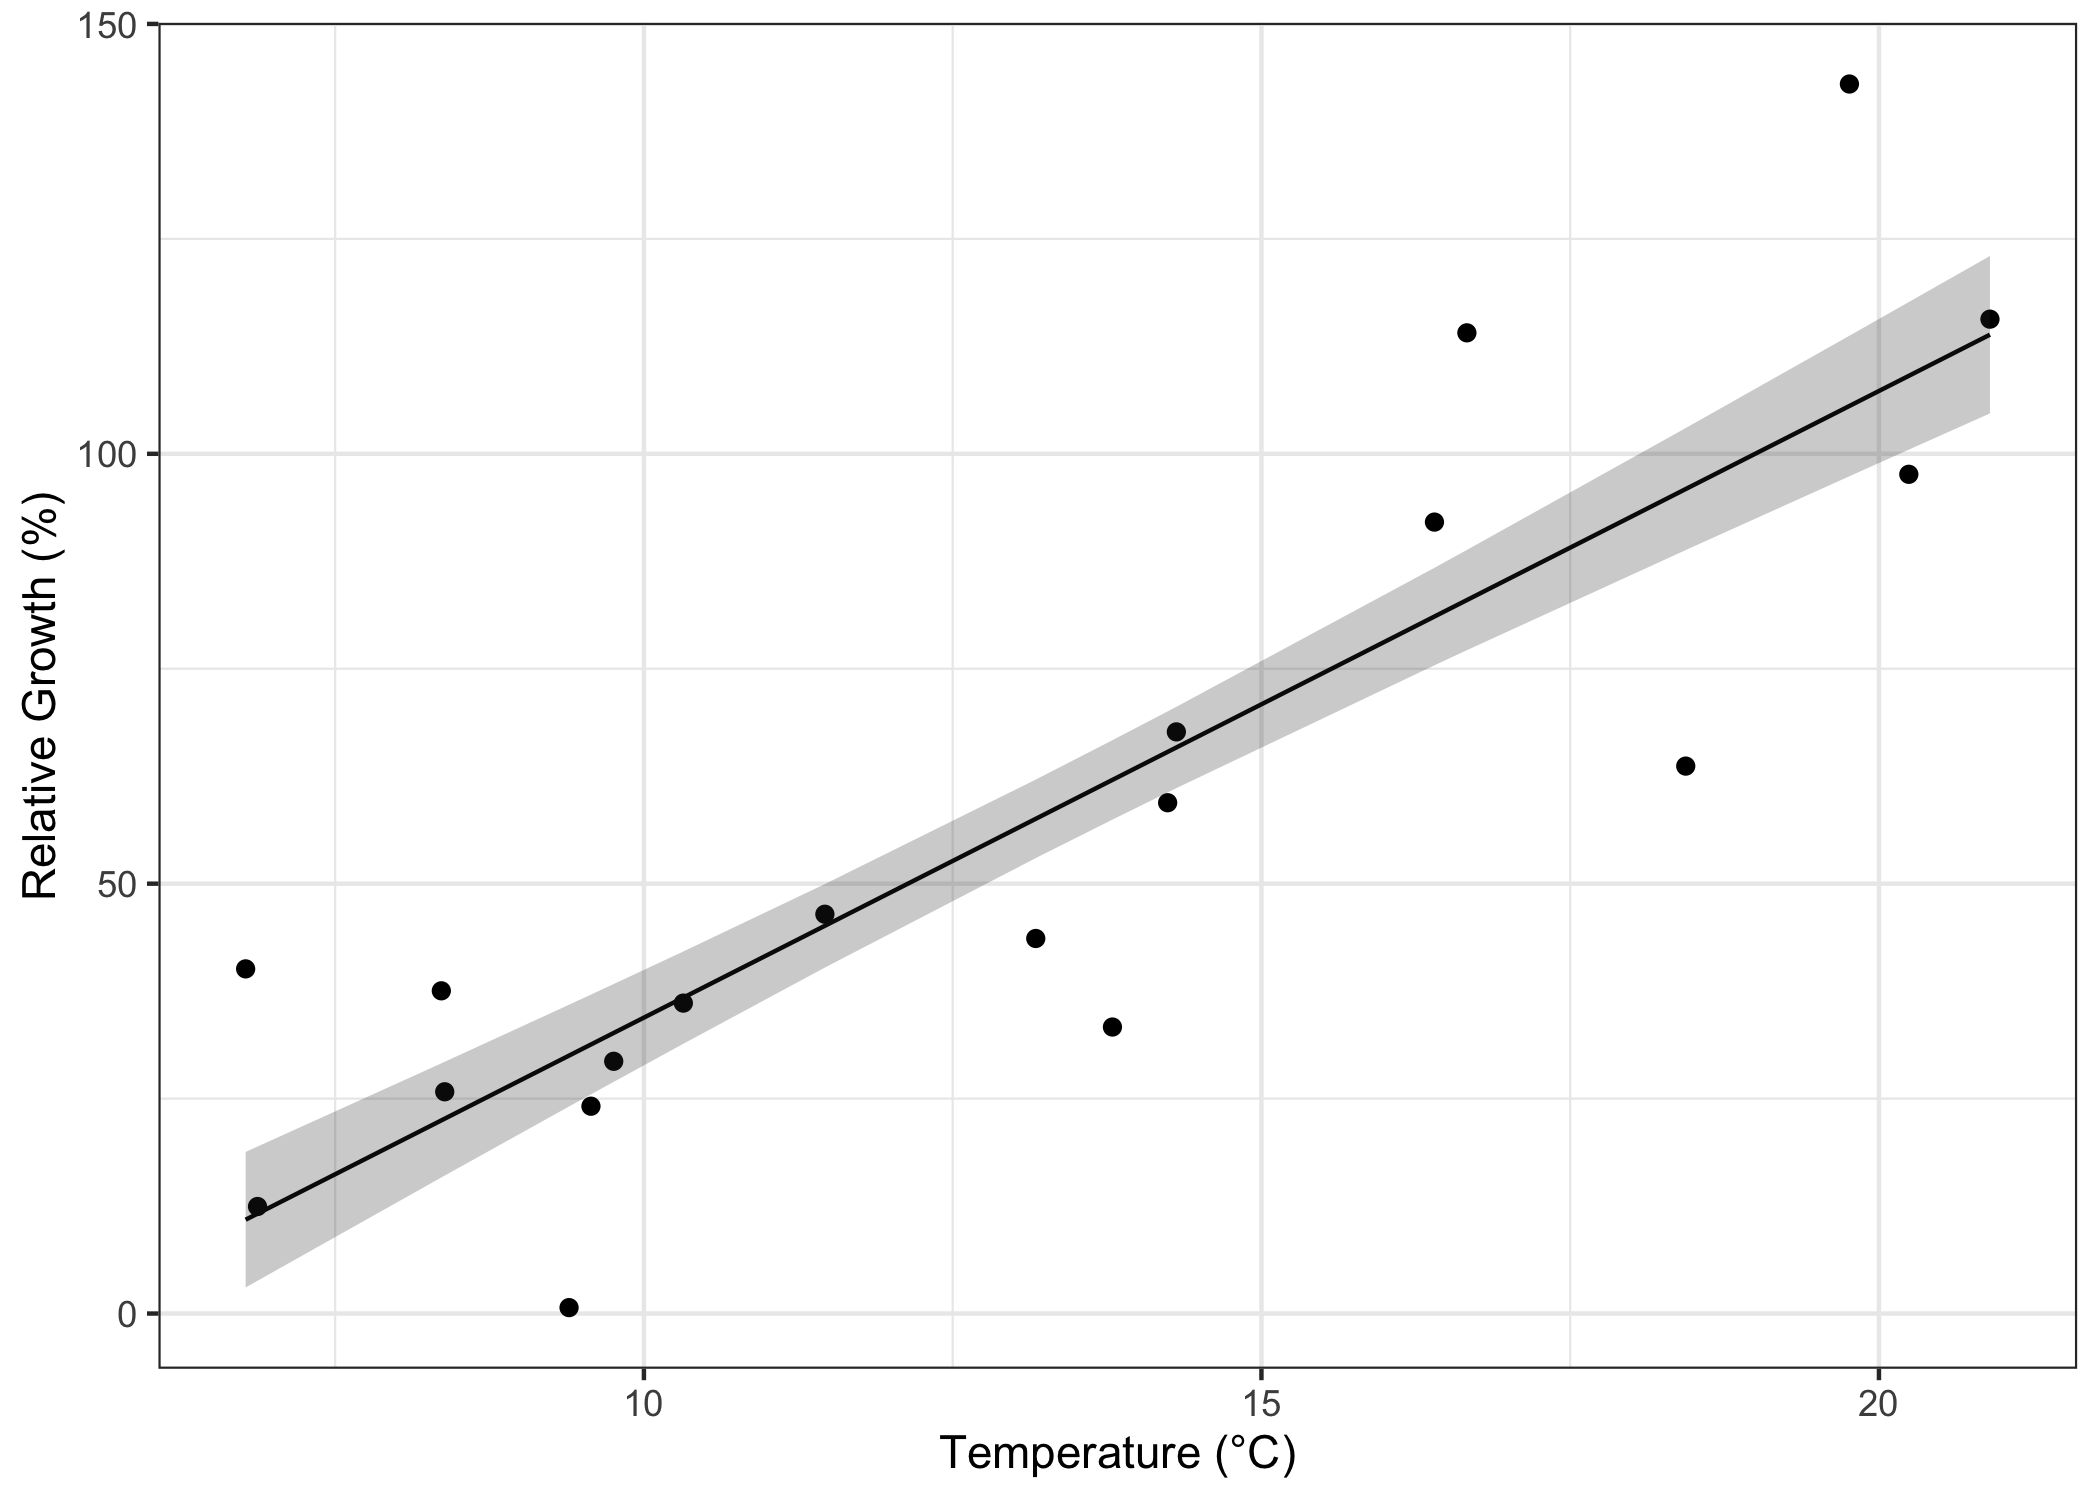
\includegraphics[width=1\linewidth]{/Users/sandraemry/Documents/Replicability_Course/Replicability-Preregistration/growth_with_temp} \caption{caption}\label{fig:growth with temp}
\end{figure}

\hypertarget{other}{%
\section{Other}\label{other}}

\hypertarget{other-optional}{%
\subsection{Other (Optional)}\label{other-optional}}

Enter your response here.

\hypertarget{references}{%
\section{References}\label{references}}

\hypertarget{section}{%
\subsection{}\label{section}}

\vspace{-2pc}
\setlength{\parindent}{-0.5in}
\setlength{\leftskip}{-1in}
\setlength{\parskip}{8pt}

\noindent

\end{document}